\documentclass{article}

\usepackage[table]{xcolor}
\usepackage{amsmath, physics, tikz, microtype, float, fancyhdr, hyperref, enumitem, siunitx, cancel}
\usepackage[letterpaper, bottom=1in, top=1in, left=1in, right=1in]{geometry}

\urlstyle{same}

\pagestyle{fancy}

\title{Report 2: Force Tables}
\date{3/3/2023}
\author{Laith Toom}

\begin{document}
\maketitle
\noindent Phys 207 Lab CD4

\noindent \textbf{Instructor:} Georgios Goulas

\noindent \textbf{Group:} Radjabov Jake and Tenzin Tsepak

\newpage 

\tableofcontents

\newpage

\section{Introduction}
\paragraph{Objective} This lab is meant to develop a deeper understanding of what 
vectors are and what it means to add vectors. For example, vectors of the same 
magnitude that are opposite to each other will cancel out, however when modeled 
in the real world with pulleys and weights, this fact holds more significance. Another
example would be when two vectors of equal magnitude, with an angle in-between them, 
point to the left while a vector pointing to the right, aligned with the midpoint 
between the two other vectors. With a specific magnitude for the third vector, 
equilibiurm will be achieved, but on paper, this does not hold as much meaning. When 
modeled in the real world however, the canceling out of forces due to equilibiurm 
and the representation of those forces using vectors is clear.  

\bigskip
\hrule 

\section{Procedure}
\subsection{Experiment 1: Sensitivity of the Instrument}
\begin{enumerate}
    \item Arrange two pulley systems, with one pan at \ang{0} and another pan 
    at \ang{180}.
    \item Place 50 grams on both pans.
    \item On one of the pans, add 1 gram and check for equilibiurm. 
    \item Find the maximum mass you can add to this pan before equilibiurm
    is lost.
    \item Record this mass in grams.
\end{enumerate}
Determine how much mass you should need to balance the forces and compare this value 
to the mass you used. Record the difference, in grams, between your experimental mass and 
the simulated mass.

\subsection{Experiment 3: Find a Function}
Set up the force table like the below diagram, where $b=\ang{5}$ and the first two pans
(1 and 2) have 50 grams placed onto them:
\begin{figure}[H]
    \centering
    \fbox{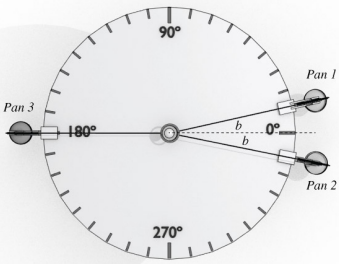
\includegraphics[width=5cm]{lab2_exp3_pic.png}}
\end{figure}

\begin{enumerate}
    \item Experiment to find the mass that should be placed on pan 3 
    such that equilibiurm is achieved.
    \item Repeat this experiment by increasing angle $b$ by \ang{5} until 
    $b=\ang{80}$ or equilibiurm cannot be achieved.
    \item Record your results in the following table:
\end{enumerate}
\begin{figure}[H]
    \centering
    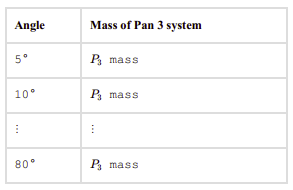
\includegraphics[width=6.5cm]{lab2_example_table.png} 
\end{figure}
Determine a function to predict the mass of pan 3 with respect to angle $b$, where the 
summed masses of pan 1 and 2 the constant $C=200\mathrm{g}$. This equation should look like:
\[ P_3(b) = C\cos(b) \]
We will then use Microsoft Excel to plot the recorded masses of pan 3 with respect to the cosine of 
the angle $b$ and plot a linear trendline. The slope of the trendline will be our constant 
$C$.

\subsection{Return to the Force Table}
Use the provided number generator to produce 3 pairs of masses and directions. Each 
pair will be the mass and direction of a vector. Then, use vector algebra to calculate 
a fourth vector $\va{D}$ such that:
\[ \va{A} + \va{B} + \va{C} + \va{D} = 0 \]
Once vector $\va{D}$ is calculated, record the values for $\abs{D_x}$ and $\abs{D_y}$.
Convert $\va{D}$ back to a mass and angle using trigonometric functions. Set up the force 
table using the masses and directions for all four vectors to see if the calculated prediction 
is correct, in which equilibiurm occurs.

\bigskip
\hrule

\section{Data and Calculations}
\subsection{Data}
\begin{table}[H]
    \centering
    \caption{Mass of Pan 3 and Angle $b$}
    \vspace{0.5em}
    \begin{tabular}{|r|r|}
        \hline
        \rowcolor{black}
        \multicolumn{1}{l}{\color{white} Mass (grams)} & \multicolumn{1}{l}{\color{white} $b$ (\textdegree)} \\
        \hline
        108\,g       & \ang{5}       \\ 
        \hline
        107\,g       & \ang{10}       \\ 
        \hline
        105\,g       & \ang{15}       \\ 
        \hline
        103\,g       & \ang{20}       \\ 
        \hline
        98\,g        & \ang{25}       \\ 
        \hline
        94\,g        & \ang{30}       \\ 
        \hline
        90\,g        & \ang{35}       \\ 
        \hline
        84\,g        & \ang{40}       \\ 
        \hline
        76\,g        & \ang{45}       \\ 
        \hline
        69\,g        & \ang{50}       \\ 
        \hline
        62\,g        & \ang{55}       \\ 
        \hline
        54\,g        & \ang{60}       \\ 
        \hline
    \end{tabular}
\end{table}

\begin{table}[H]
    \centering
    \caption{Mass of Pan 3 and $\cos(b)$}
    \vspace{0.5em}
    \begin{tabular}{|r|r|}
        \hline
        \rowcolor{black}
        \multicolumn{1}{l}{\color{white} Mass (grams)} & \multicolumn{1}{l}{\color{white} $\cos(b)$} \\
        \hline
        108\,g           & 0.9961947       \\ 
        \hline
        107\,g           & 0.98480775       \\ 
        \hline
        105\,g           & 0.96592583       \\ 
        \hline
        103\,g           & 0.93969262       \\ 
        \hline
        98\,g           & 0.90630779       \\ 
        \hline
        94\,g           & 0.8660254       \\ 
        \hline
        90\,g           & 0.81915204       \\ 
        \hline
        84\,g           & 0.76604444       \\ 
        \hline
        76\,g           & 0.70710678       \\ 
        \hline
        69\,g           & 0.64278761       \\ 
        \hline
        62\,g           & 0.57357644       \\ 
        \hline
        54\,g            & 0.5      \\ 
        \hline
    \end{tabular}
\end{table}

\begin{figure}[H]
    \caption{Mass of Pan 3 as a Function of $cos(b)$}
    \vspace{0.5em}
    \centering
    \fbox{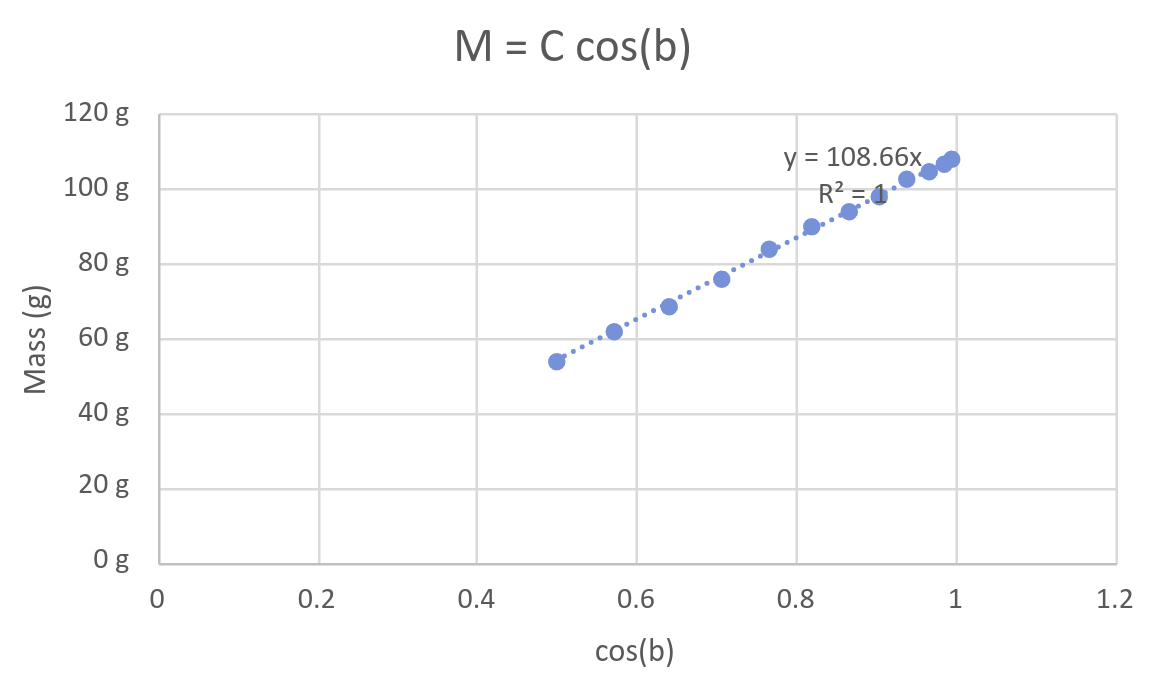
\includegraphics[width=13cm]{lab2_plot1.png}}
\end{figure}

\subsection{Calculations}
\subsubsection{Calculating $\va{D}$}\label{calcD}
Since we have the equation:
\[ \va{A} + \va{B} + \va{C} + \va{D} = 0 \]
this implies that:
\[ \va{A} + \va{B} + \va{C} = -\va{D} \]
thus:
\[ D_x = -(A_x+B_x+C_x) \qquad \text{and} \qquad D_y = -(A_y+B_y+C_y)  \]
Since we are looking for the magnitudes of $D_x$ and $D_y$, this equation becomes:
\[ \abs{D_x} = \abs{A_x+B_x+C_x} \qquad \text{and} \qquad \abs{D_y} = \abs{A_y+B_y+C_y}  \]
We can draw this as a force diagram, where the origin is the center of the 
force table:
\begin{figure}[H]
    \centering
    \begin{tikzpicture}[scale=1.2]
        \draw[stealth-stealth] (0, -3) -- (0, 3) node[above]{$y$};
        \draw[stealth-stealth] (-3, 0) -- (3, 0) node[right]{$x$};
        \draw[-stealth, blue] (0, 0) -- (-1.5, 1.5) node[above]{$\va{B}$}; 
        \draw[-stealth, blue] (0, 0) -- (-2, 0) node[above]{$\va{A}$}; 
        \draw[-stealth, blue] (0, 0) -- (2, 0) node[above]{$\va{C}$}; 
        \draw[-stealth, red] (0, 0) -- (2, -2) node[below right]{$\va{D}$}; 

        \draw (-1, 1) arc (120:187:1) node[above left, midway] {$\alpha=\ang{45}$};

        \node[scale=3] at (0, 0) {$.$};
    \end{tikzpicture}
\end{figure}
We can see that $\va{A}$ and $\va{C}$ do not have $y$-components, but all three 
vectors have $x$-components. We can calculate the $x$-component of $\va{D}$ by taking the 
magnitudes of $\va{A}$, $\va{C}$, and $B_x$. The magnitude of $B_x$ will equal:
\[ B_x = -\abs{\va{B}}\cos(\alpha) = -70g\cos(\ang{45}) \quad \text{$\va{B}$ exerts a 
negative force along $x$}\]
where $g$ is acceleration by gravity (9.8 m/s$^2$) and 70 is the mass of the object applying force 
$\va{B}$ to the center of the force table. The magnitudes of $\abs{\va{A}}$ and $\abs{\va{C}}$ are:
\begin{align*}
    &\abs{\va{A}} = -M_Ag = -70g \quad \text{$\va{A}$ exerts a negative force along $x$.}\\
    &\abs{\va{C}} = M_Cg = 80g 
\end{align*}
Thus:
\[ \abs{D_x} = \abs{-70g+80g-70g\cos(45)} \approx 0.387\,\mathrm{N} \]
Since $\va{A}$ and $\va{C}$ do not have $y$-components, the only value needed to 
calculate $\abs{D_y}$ is $B_y$. $B_y$ will equal:
\[ B_y = \abs{\va{B}}\sin(\alpha) = 70g\sin(45) \]
thus:
\[ \abs{D_y} = \abs{70g\sin(45)} \approx 0.485\,\mathrm{N} \]
We can calculate $\abs{\va{D}}$ to be:
\[ \abs{\va{D}} = \sqrt{D_x^2 + D_y^2} \approx 0.385\,\mathrm{N} \]
since $\mathrm{N}=\mathrm{kg\cdot m/s^2}$, we can multiply by 1000 and divide by gravity 
in order to get the analytical mass required to achieve equilibiurm:
\[ 0.385\,\cancelto{\mathrm{g}}{\mathrm{kg}}\cdot \cancel{\mathrm{m/s^2}} \cdot 1000 \cdot \frac{1}{9.8\,\mathrm{m/s^2}} \approx 39.29\,\mathrm{g}\]
    
\bigskip
\hrule

\section{Questions}
\subsection*{\normalsize(1) What factors could contribute to this sensitivity?}
Regarding the sensitivity of the force table, the friction between the rope 
and the pulley wheel could contribute to this sensitivity. More friction would 
require more weight to lose equilibiurm, thus making the force table less 
sensitive. Less friction would have the opposite effect, making the force table 
more sensitive.

\subsection*{\normalsize(2) Report the difference between what you've experimentally measured and 
what the simulation predicted. Are they within the expected sensitivity of the 
instrument?}
The difference between my experimental mass and the simulated mass was $5.46\pm0.5\mathrm{g}$
since the experimental mass of the resultant was $79.9\pm0.5\mathrm{g}$ and the simulated mass 
was $85.6\pm0.5\mathrm{g}$. This is within the expected sensitivity of the instrument since we 
experimentally determined the sensitivity to be $5.0\pm0.5\mathrm{g}$.

\subsection*{\normalsize(3) On one graph plot the experimental data from your table along with the 
analytical prediction of the function you found. Do they follow the same trend?
Then, find the slope of your linear data and compare it to what the slope should be from 
your analytical equation. Does it differ from the analytically derived slope by less 
than the uncertainty?}
The experimental data and the analytical prediction follow the same trend, in which both 
are linear functions. The slope of the linear data was 109.95 grams, and the analytical equation had a slope of 
200 grams. However, considering that both pans had 50 grams placed onto them, those grams 
could cancel out, and the slope could be 100. Since the sensitivity of our force table of two
and our slope should theoretically equal the sum of the masses of the two pans:
\[ P_3(b) = C\cos(b) \quad \text{where} \quad C=P_1+P_2 \]
the uncertainty in this case will be the sensitivity of our force table multiplied by two to
account for sensitivity of the masses two pans we are using:
\[ \delta P = 5.0\pm0.5\,\mathrm{g}\cdot 2 = 10.\pm1.0\,\mathrm{g} \]
Thus, experimentally derived slope could differ from the analytically derived slope by 
less than the uncertainty if we consider the analytical slope to be 100 grams. However, 
since the analytical slope was originally 200 grams, then the difference between the 
experimentally derived slope and analytical slope is greater than our uncertainty.

\subsection*{\normalsize(4) Give the details of this calculation and compare your analytical results 
with the the experimental results. Draw a vector diagram that shows the table arrangement.}
Analytically, we found that a mass of 39.29 grams for the fourth pan would be required to 
reach equilibiurm. Experimentally, we found that adding 35 grams to the fourth pan would 
reach equilibiurm. With a difference of 4.29 grams, the two values differ by less than 
the uncertainty of the force table, which was found to be $5.0\pm0.5\mathrm{g}$. 

\bigskip 
\hrule 

\section{Conclusion}
\paragraph{Error} The room for error in this lab could be due the force table being 
slightly off from the provided setup. For example, when calculating $D_x$ and $D_y$ in section 
\ref{calcD}, our provided direction for vector $\va{B}$ was \ang{55}, but when setting up the 
pulley system at that angle, we we might have set up a direction of \ang{54} of \ang{56}. The same 
could apply to weight, where not placing the weights exactly on top of each other, or centered perfectly, 
could alter the center of mass for the pans, thus the vectors we set up would have different magnitudes 
than the analytical vectors. We also have to take into the account the sensitivity of the force table, which
could present significant gaps between the experimental values and analytical values. 
With this potential error occuring in four vectors, our experimental observation would not match exactly with the 
analytical value.

There is also possibility of not accounting for the inherent masses of the pans, which are 50 grams.
With a significant mass, not accounting for it by mistake or misunderstanding would produce major 
errors in experimental and analytical results.

\paragraph{Findings} A greater angle between two vectors decreases the magnitude of the 
resultant. This helps to explain why when the angle between vectors is \ang{180}, in which 
the vectors are opposite to each other, there is no resultant, or that the magnitude of the 
resultant is 0 N.

\paragraph{Revisions} Perhaps using pans with insignficant masses, such as masses around 
1 gram, would make the experiment more clear and cut down on potential errors. Although the 
masses should theoretically cancel out in a state of equilibiurm, mistakenly not accounting for 
them would produce large errors, such as when experimentally deriving the slope for experiment 3. 

\end{document}